\vspace{.25cm}
\begin{figure}[ht!]
\centering
	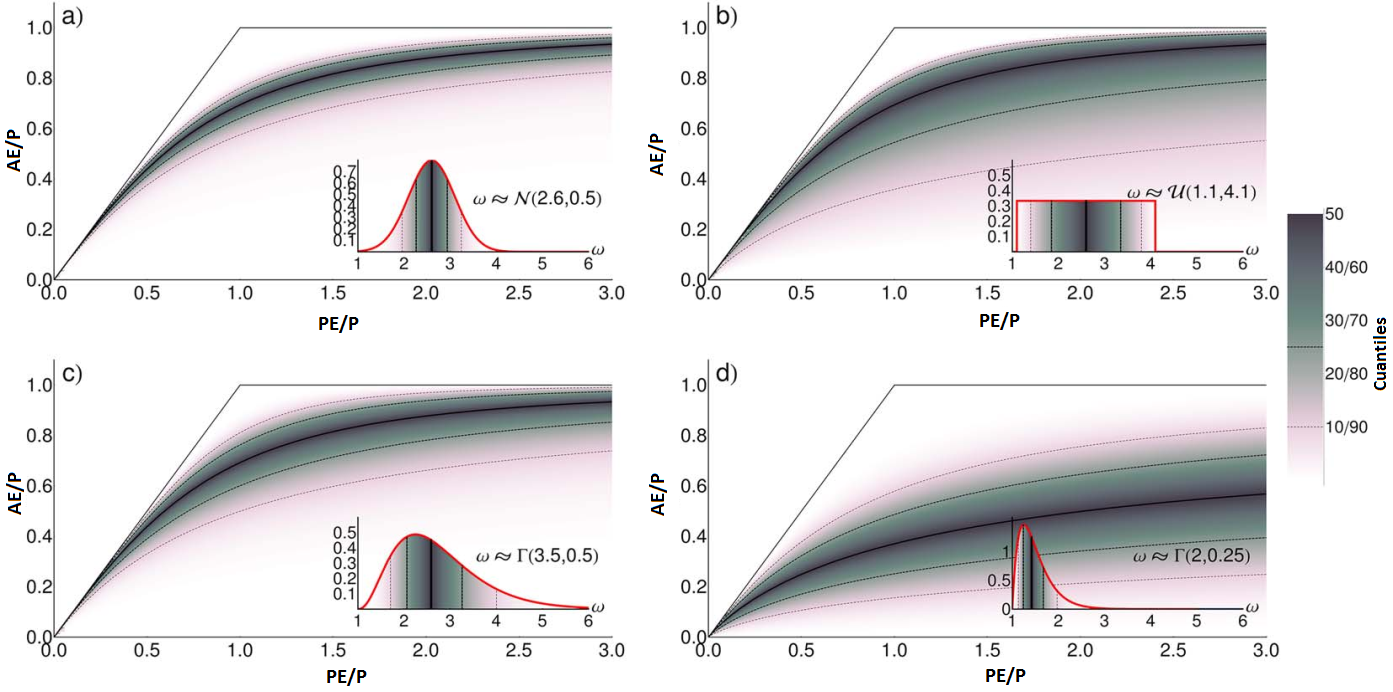
\includegraphics[scale=0.35]{Images/Greve02.png}
	\caption{Enfoque de Budyko probabilístico con un $\omega$ siguiendo a) una distribución normal truncada, b) una distribución uniforme y (c y d) dos diferentes distribuciones gamma. Las distribuciones de a, b y c muestran una mediana comuna $\omega = 2.6$, que corresponde al Budyko original (linea negras solida). Los respectivos cuantiles se muestran como sombras.}
	Fuente: \citet{Greve2015}.
	\label{fig:Greve02}
\end{figure}